\chapter{Introducció}
\section{Presentació del treball}
\par La concepció d'aquest treball sorgeix de l'interès de l'autor per l'electrònica digital i analògica, i de demostrar les avantatges d'implementar sistemes que es beneficiïn dels dos vessants. Es planteja doncs el disseny i implementació d'un amplificador d'àudio de tipus D, que com es comentarà més endavant, es poden obtenir altes prestacions a la sortida amb tècniques de processament digital.  
\par La tecnologia d'àudio digital està substituint progressivament la majoria dels dispositius i tasques que tradicionalment es duien a terme amb components analògics. Aquesta tecnologia es pot considerar com una evolució de les pràctiques i tècniques desenvolupades durant dècades en l'àmbit de l'electroacústica i l'enginyeria d'àudio. Tot i això, la conversió digital dels senyals comporta el risc de pèrdues significatives en la qualitat del so si no es prenen les mesures adequades. Mitjançant tècniques com el filtratge i el modelatge del soroll, és possible obtenir una qualitat d'àudio elevada de manera eficient. A més, el processament digital de senyals ofereix avantatges significatius respecte al tractament analògic, especialment pel que fa a la reducció del consum energètic, fet que el converteix en una alternativa més sostenible i eficient en molts casos. 
\par Per a la implementació de sistemes de processament digital de senyals (DSP), l’ús de FPGAs (Field-Programmable Gate Arrays) es presenta com una de les millors opcions. Les FPGAs permeten una flexibilitat i paral·lelisme que són difícils d’assolir amb altres arquitectures, com ara microprocessadors o DSPs dedicats. Aquesta característica les fa especialment adequades per a aplicacions on es requereix un alt rendiment en temps real, com ara en sistemes d'àudio digital. A més, les FPGAs permeten personalitzar l'arquitectura per optimitzar l'ús de recursos i el consum energètic, adaptant-se de manera òptima als requisits específics del projecte. Per aquestes raons, les FPGAs són una eina clau en el desenvolupament d’amplificadors d’àudio de tipus D, ja que poden gestionar amb precisió la modulació i el filtratge digital, garantint unes prestacions excel·lents tant en eficiència com en qualitat sonora.

\par Mitjançant l'ús de tècniques avançades de processament digital de senyals, es pretén aconseguir un sistema altament eficient, amb un consum energètic reduït i unes prestacions acústiques de qualitat elevada. A més, es posa èmfasi en la versatilitat d'aquests sistemes i en la seva capacitat per superar els límits dels enfocaments exclusivament analògics o digitals. Finalment, en aquest treball es dissenyarà una etapa de recepció d'àudio en protocol I2S, una etapa de filtratge i un modulador $\Sigma \Delta$ amb l'objectiu de fer sonar uns auriculars amb un so nítid.

\section{Objectius}
\par Per a la realització d'aquest treball es defineixen els següents objectius amb la intenció d'implementar una etapa completa d'àudio funcional i adquirir coneixements en la matèria de processament digital de senyals. A continuació s'enumeren els objectius que s'ha fixat en la realització d'aquest treball.
\begin{itemize}
    \item Objectiu 1: Implementar un bloc IP receptor per fer lectures en protocol I2S.
    \item Objectiu 2: Dissenyar i implementar etapes de filtrat per l'àudio a l'entrada i sobremostrejar el senyal.
    \item Objectiu 3: Dissenyar i implementar un modulador $\Sigma \Delta$ que modeli el soroll provocat per la quantificació.
    \item Objectiu 4: Dissenyar una etapa de delmat del senyal d'àudio provinent del bloc $\Sigma \Delta$.
\end{itemize}
\par En la valoració final del que s'acabi implementant, es farà un incís per analitzar si s'han complert tots els objectius. 

\section{Amplificadors d'àudio de Classe D}
\par Els amplificadors de classe D són una topologia d'amplificadors electrònics dissenyats per oferir una gran eficiència energètica on els transistors de l'etapa de sortida treballen en règim de commutació i no en règim lineal. En el nivell més elemental de la teoria, l'eficiència d'un amplificador de classe D sempre és del 100\%, a tots els nivells de sortida. A la pràctica, les idealitzacions matemàtiques no es mantenen, i l'eficiència a la vida real dels amplificadors de classe D cau en fins al 80 i 90 \% en la major part del rang de potència a la sortida. Aquestes pèrdues s'originen per diferents mecanismes: 

\begin{itemize}
	
	\item Pèrdues en els transistors a la sortida: Els transistors de l'etapa de sortida tenen una resistència de conducció no nul·la quan estan en règim de saturació, fet que origina pèrdues per $I^{2}R$. A més a més, s'afegeixen les pèrdues per commutació que es veuen agreujades pels components paràsits en els FET.
	
	\item Polsos de retrocés: Degut a la naturalesa inductiva de la càrrega, durant les transicions de nivell es genera una variació del flux magnètic a la bobina, la qual dona lloc a fenòmens transitoris. Aquests fenòmens poden activar els díodes paràsits inherents als FET, provocant la seva conducció no desitjada. Aquests díodes, amb un temps de recuperació inversa relativament llarg, permeten la circulació d’un corrent superior al necessari, cosa que pot afectar l’eficiència del sistema i incrementar les pèrdues energètiques.
	
	\item Shoot-through: Aquest terme fa referència a la situació en què els dos transistors d'un semipont estan conduint al mateix temps. Això provoca un curtcircuit gairebé directe entre els raïls d’alimentació. Per evitar-ho, el circuit de control dels transistors incorporen un temps mort entre transicions de conducció.
	
\end{itemize}

\par El senyal d'àudio d'entrada es modula en un senyal de control digital que impulsa els dispositius de potència a l'etapa de sortida. Aquest senyal es pot modular, normalment, mitjançant modulació d'amplada de pols (PWM) o modulació de densitat de pols (PDM).

\par L'etapa de sortida es pot implementar mitjançant una topologia de Half-Bridge o Full-Bridge, il·lustrada a les figures \ref{fighalfbridge} i \ref{figFullbridge}. Els amplificadors de classe D sovint funcionen en una configuració de pont per augmentar la potència de sortida sense augmentar les tensions d'alimentació. L'última etapa, el filtre de pas baix, s'utilitza per eliminar la freqüència portadora PWM/PDM d'alta freqüència, recuperant així el senyal d'àudio original\cite{SDMClassD}.
\begin{figure}[H]
    \centering
    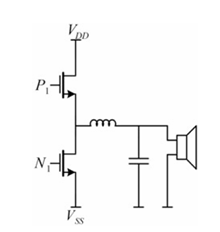
\includegraphics[width=0.25\linewidth]{Images/halfbridge.png}
    \caption{Amplificador de classe D en configuració de semi-pont.}
    \label{fighalfbridge}
\end{figure}
\begin{figure}[H]
    \centering
    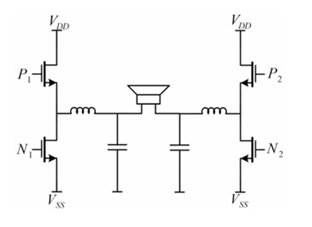
\includegraphics[width=0.3\linewidth]{Images/full-bridge.png}
    \caption{Amplificador de classe D en configuració de pont complet.}
    \label{figFullbridge}
\end{figure}

\subsubsection{Amplificadors de Classe D comercials}
\par En aquest apartat es presenten amplificadors de classe D i DSPs units disponibles en el mercat, i es desglossen les prestacions més rellevants.
\begin{itemize}
    \item AX5688: Amplificador digital de classe D amb entrada d'àudio en protocol I2S, etapa de filtrat i etapa de potència, integrat en el mateix IC. Té 2 sortides PWM que es poden configurar per atacar 2 altaveus en configuració semi-pont o un altaveu en pont complet. Rang Dinàmic = 115 dB; THD+N = -100 dB. \cite{MPSAmpD}
    \item TAS2320: Amplificador digital de classe D amb entrad mono en protocol I2S i etapa de potència de 15 W. L'etapa de potència només pot atacar un altaveu en configuració de semi-pont. Rang Dinàmic = 109dB; THD+N = -89 dB. \cite{TIAmpD}
    \item MAX98365: Amplificador digital de classe D mb entrada d'àudio en protocol I2S i etapa de potència fins 17.6 W. L'etapa de potència només pot atacar un altaveu en configuració de semi-pont. Rang Dinàmic = 111,5 dB; THD+N = -85 dB.\cite{AnalogAmpD}
\end{itemize}

\section{FPGA}
\par Les FPGA són circuits integrats (IC) d'integració a gran escala (VLSI) que poden contenir centenars de milers de blocs lògics configurables (CLB), desenes de milers de blocs funcionals de maquinari predefinits, centenars d'interfícies externes predefinides, milers de blocs de memòria, milers de pads d'entrada/sortida (I/O) i fins i tot un SoC totalment predefinit en determinades famílies FPGA. Aquests elements funcionals es distribueixen de manera òptima per l'àrea de silici de la FPGA i es poden interconnectar mitjançant recursos d'encaminament programables. Això els permet comportar-se d'una manera funcional desitjada per un dissenyador lògic de manera que puguin complir determinades especificacions de disseny i requisits del producte. \cite{Maaref2023} 
\begin{figure}[H]
    \centering
    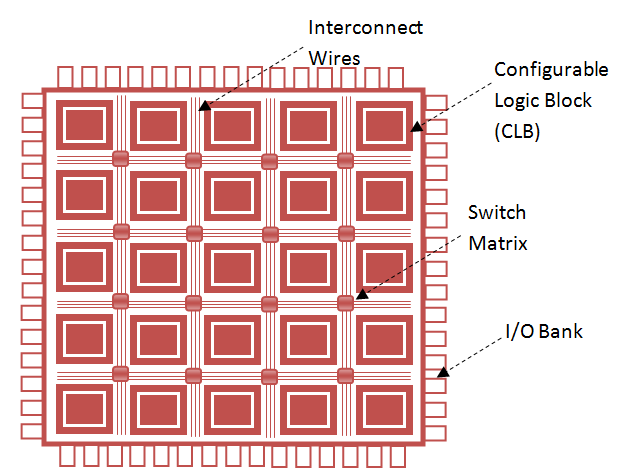
\includegraphics[width=0.5\linewidth]{Images/FPGAdiagram.png}
    \caption{Diagrama de blocs dels elements en una FPGA en el silici del IC.}
    \label{figFPGA}
\end{figure}
\par A diferència dels processadors, els FPGA són capaços de fer operacions paral·leles, de manera que diferents operacions de processament no competeixen pels mateixos recursos. Cada tasca independent s'assigna a una secció dedicada del xip i pot funcionar de manera autònoma sense influència d'altres blocs lògics. En conseqüència, el rendiment d'una part de l'aplicació no es veu afectat a mesura que s'afegeixen més operacions.
\par Les FPGA contenen components especialitzats per a funcions específiques i una lògica configurable de propòsit més general. A continuació es mencionen alguns d'aquests blocs que caracteritzen les FPGAs \cite{FPGADig}:
\begin{itemize}
    \item Configurable Logic Block (CLB): Els blocs lògics configurables (CLB) són la unitat lògica bàsica d'un FPGA. Un CLB dóna a l'FPGA la seva capacitat d'acceptar diferents configuracions de maquinari. Els CLB es poden programar per realitzar gairebé qualsevol funció lògica. El CLB individual conté una sèrie de components lògics discrets, com ara taules de consulta (LUT) i flip-flops.
    \item Flip Flops: Un flip-flop és un circuit que té dos estats estables i es pot utilitzar per emmagatzemar informació. Els flip-flops són registres de desplaçament binaris que sincronitzen la lògica i guarden estats lògics entre cicles de rellotge dins d'un circuit FPGA. Un flip-flop emmagatzema un sol bit de dades.
    \item Look Up Tables (LUT): Determina quina és la sortida per a qualsevol entrada donada. En el context de la lògica combinatòria, és la taula de veritat i defineix com es comporta la lògica combinatòria. Una taula de veritat és una llista predefinida de sortides per a cada combinació d'entrades. El LUT conté una taula de veritat personalitzada que es carrega quan el xip s'engega.
    \item Blocs DSP o MAC: Realitza funcions de processament de senyal digital, com ara filtrar o multiplicar, de manera més eficient que utilitzar molts CLB. Aquest circuit multiplicador estalvia l'ús de LUT i flip-flop en aplicacions de processament de senyal i matemàtiques.
\end{itemize}

\subsubsection{Placa de desenvolupament Nexys4}
\par Pel desenvolupament del projecte i la implementació final, s'ha emprat la placa de desenvolupament Nexys4. La placa inclou la FPGA Artix-7 de Xilinx i múltiples prestacions per diverses aplicacions. A la taula \ref{taulaArtix7} es poden veure plasmades les característiques de la FPGA Artix-7. Per l'aplicació d'aquest treball, destaca l'etapa de filtrat actiu analògica, implementada amb un filtre passabaixos de 4rt ordre en topologia Sallen-Key a la sortida d'àudio en format stereo.
\begin{table}[H]
    \centering
    \begin{tabular}{ | c | }
    \hline
    \textbf{Prestacions FPGA Artix{-}7} \\ [2ex]
    \hline
    101440 LUTs \\ 
    \hline
    126800 CLBs \\ 
    \hline
    1,2 Mb RAM distribuida \\ 
    \hline
    240 blocs DSP \\ 
    \hline
    135 BRAM (FIFO) de 35 Kb \\ 
    \hline
    6 MMCM + 6 PLL \\ 
    \hline
    300 GPIOs \\ 
    \hline 
    \end{tabular}
    \caption{Recursos disponibles de la FPGA utilitzada en la placa de desenvolupament Nexys4.\cite{NEXYS4Dig}}
    \label{taulaArtix7}
\end{table}

\begin{figure}[H]
    \centering
    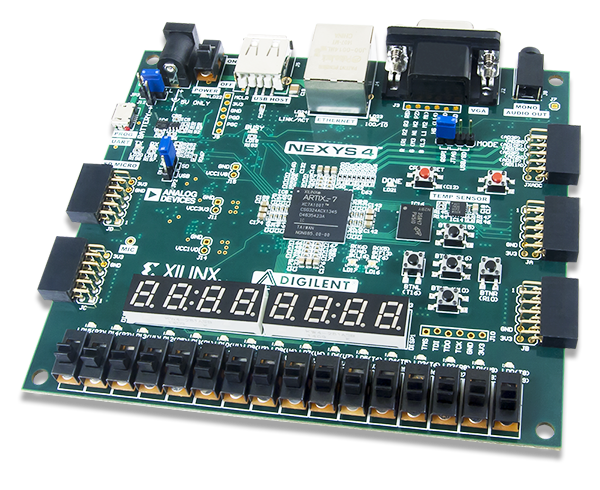
\includegraphics[width=0.3\linewidth]{Images/nexys-4.png}
    \caption{Placa de desenvolupament Nexys4 utilitzada pel desenvolupament d'aquest treball.\cite{NEXYS4Dig}}
    \label{figNEXYS4}
\end{figure}